\documentclass[french]{article}
\usepackage{babel}
\usepackage[utf8]{inputenc}
\usepackage[T1]{fontenc}
\usepackage{graphicx}
\usepackage{layout}
\usepackage[top=2cm, bottom=2cm, left=1cm, right=1cm]{geometry}
\usepackage{color}
\usepackage{amsmath,amsfonts,amssymb}
\usepackage{caption}

\title{Mesures à distances \\ Devoir Maison 2}
\author{PIPERAU Yohan \\ BELLA Jean-Paul}
\begin{document}
\maketitle
\newpage

\section*{\begin{center}
TP1 : Mesures fréquentielles en modulation d'amplitude à double bande latérale avec porteuse : DBAP (Serveur 6)
\end{center}}

\paragraph{Question 1} : \\
%\includegraphics[scale=•]{•}
Nous observons bien trois raies sur le spectre donné sur la figure 1:
\begin{itemize}
\item une raie centrale d'amplitude $A_{1}=25$mV
\item deux raies latérales d'amplitude $A_{2}=A_{3}=6$mV
\end{itemize}
\paragraph{Question 2} : \\
Le taux de modulation m est donnée par la relation :
\begin{equation*}
m=\frac{V_{max}-V{min}}{V_{max}+V{min}}=\frac{A_{2}-A_{1}}{A_{2}+A_{1}}=0.61
\end{equation*}
\paragraph{Question 3} : \\
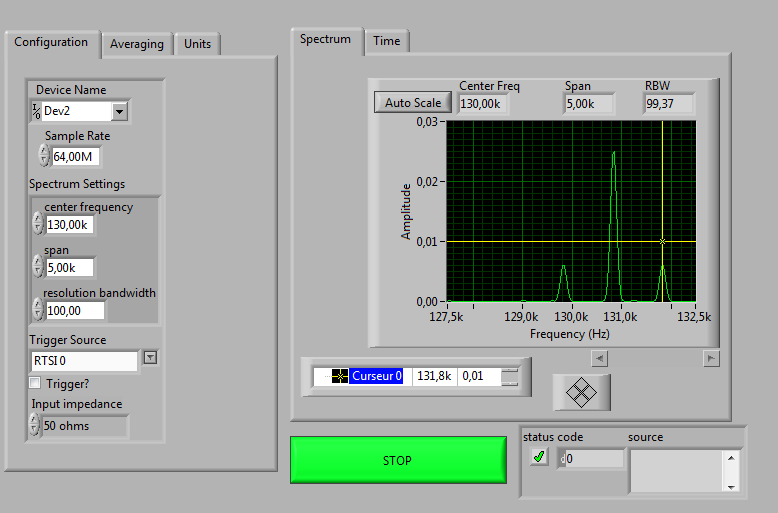
\includegraphics[width=\textwidth]{DM2_fig3.png}
Les fréquences des ondes sont visibles sur la figure 1 donnée à la question 1. \\
L'onde porteuse possède une fréquence $f_{p} = 130.8$kHz.  \\
Les raies latérales ont pour fréquences $f_{1}=129,8$kHz et $f_{2}=131.8$kHz.
\paragraph{Question 4} : \\
\begin{center}
 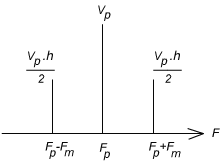
\includegraphics[width=150px]{DM2_fig2.png}
 \end{center} 
Comme on le voit sur la figure 2, nous pouvons remonter à la fréquence $f_{m}$ du message.
$f_{1}=f_{p}-f_{m}$ et $f_{3}=f_{p}+f_{m}$, d'où :
\begin{equation*}
f_{m}=\frac{f_{3}-f_{1}}{2}=1kHz
\end{equation*}
\paragraph{Question 5} : \\
\begin{center}
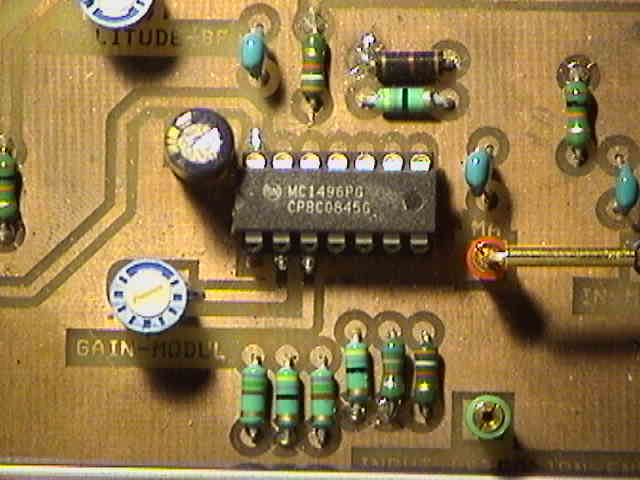
\includegraphics[width=300px]{DM2_Q5.jpg} 
\end{center}
Le nom du circuit lisible sur la 1ère ligne de caractères est : MC1496PG. \\
C’est un microcontrôleur qui envoie en sortie une tension égale au produit d’une tension d’entrée et d’une fonction de switching.

\paragraph{Question 6} : \\
Nous avons opté ici pour une modulation à double bande latérale avec porteuse. Le principe ce cette modulation est de permettre la transposition du signal modulant (message) autour de notre fréquence porteuse $f_{p}$.\\ La bande passante B du signal modulé est alors égale au double de la bande passante du signal modulant : c'est pourquoi on parle de modulation à double bande latérale. \\
Le signal est produit par multiplication, ce qui explique le recours au microcontrôleur évoqué à la question précédente.\\

Le principal inconvénient de cette méthode est de transporter la plus grande partie de son énergie dan la porteuse, alors que l'information se situe dans les bandes latérales. Elle reste toutefois plus simple à mettre en place que la modulation d'amplitude à double bande sans porteuse, c'est pourquoi elle reste encore de nos jours très largement utilisée.


\section*{\begin{center} TP2 : Mesures temporelles en modulation d'amplitude à double bande latérale avec porteuse : DBAP   (Serveur 5) \end{center}}

\paragraph{Question 2} : \\
On mesure l’amplitude de l’onde en mesurant l’amplitude crête à crête et en divisant par deux. \\
Les amplitudes $A_{m}$ et $A_{p}$ des signaux $f_{m}$ et $f_{p}$ sont respectivement 858mV et 1.75V.\\

\paragraph{Question 3} : \\
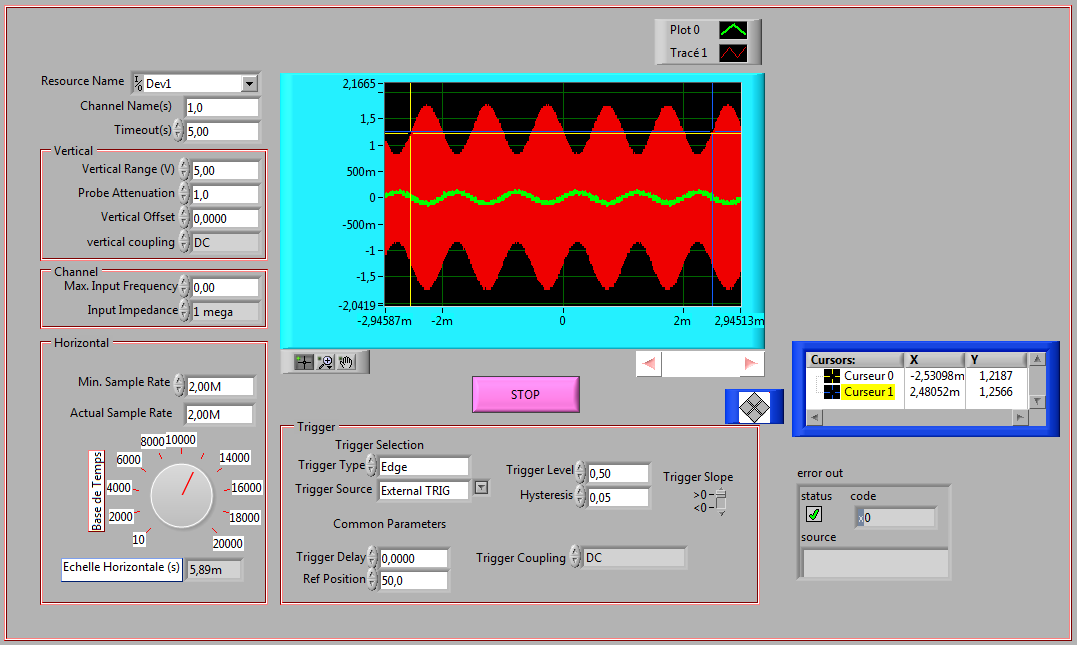
\includegraphics[width=\textwidth]{hello.png}
La fréquence $f_{p}$ de la porteuse est de 1kHz. 


\paragraph{Question 4} : \\
Afin de remonter à la fréquence $f_{m}$ du signal, nous pouvons compter cinq périodes sur le graphique pour trouver $5T_{m}=5.10^{-3}$s, ce qui correspond bien à $f_{m}=\frac{1}{T_{m}}=1$kHz (d'après le réglage réalisé en question 1).


\section*{\begin{center} TP3 : Mesures en démodulation d'amplitude à double bande latérale avec porteuse : DBAP (serveur 4) \end{center}}

\paragraph{Question 2} : \\
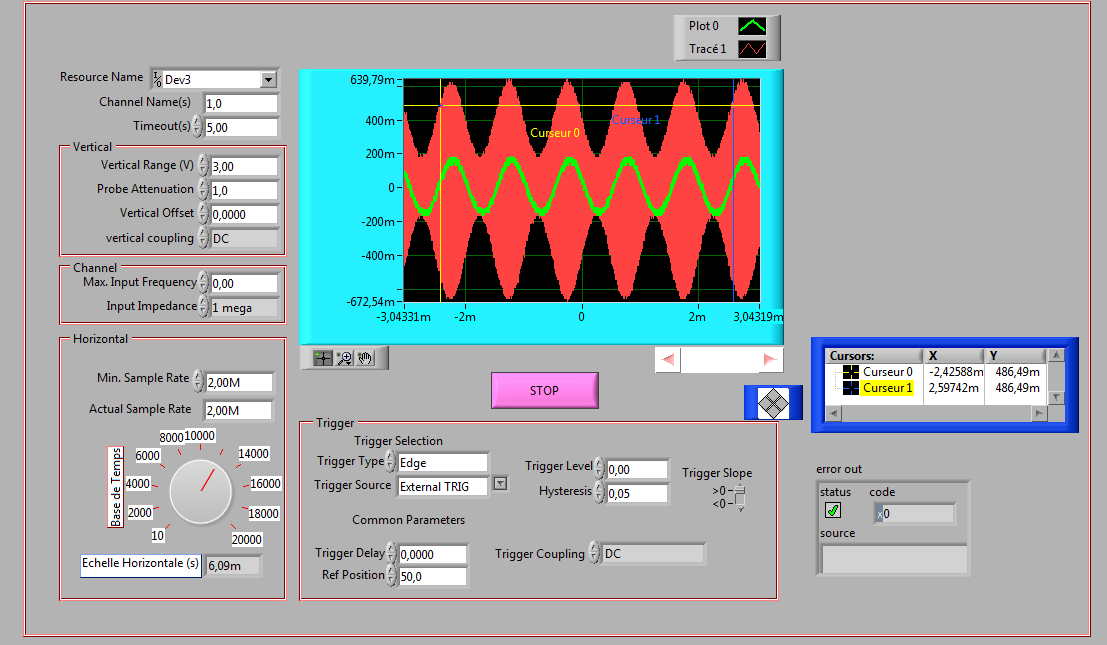
\includegraphics[width=\textwidth]{bonjour.png}

On mesure les amplitudes de l'enveloppe et du message qui sont respectivement de $A_{max}=647$mV et de $A_{min}=177$mV. \\
Ainsi, on trouve \textbf{m=0.57}.

\paragraph{Question 3} : \\
La fréquence $f_{p}$ de la porteuse est de 1kHz (obtenue avec les mêmes méthodes que précédemment).
\paragraph{Question 4} : \\
L'amplitude crête à crête $V_{env}$ du signal démodulé est de 342 mV.\\
Sa fréquence $f_{m}$ est de 0.94kHz environ.
\paragraph{Question 5} : \\
Maintenant, l'amplitude crête à crête $V_{syn}$ du signal démodulé est de 133mV.\\
Sa fréquence $f_{m}$ est de 1kHz.
\paragraph{Question 6} : \\
On passe désormais en surmodulation (m>1). \\
Distinguons les deux situations suivantes : \\
\begin{itemize}
\item détecteur d'enveloppe :  \\
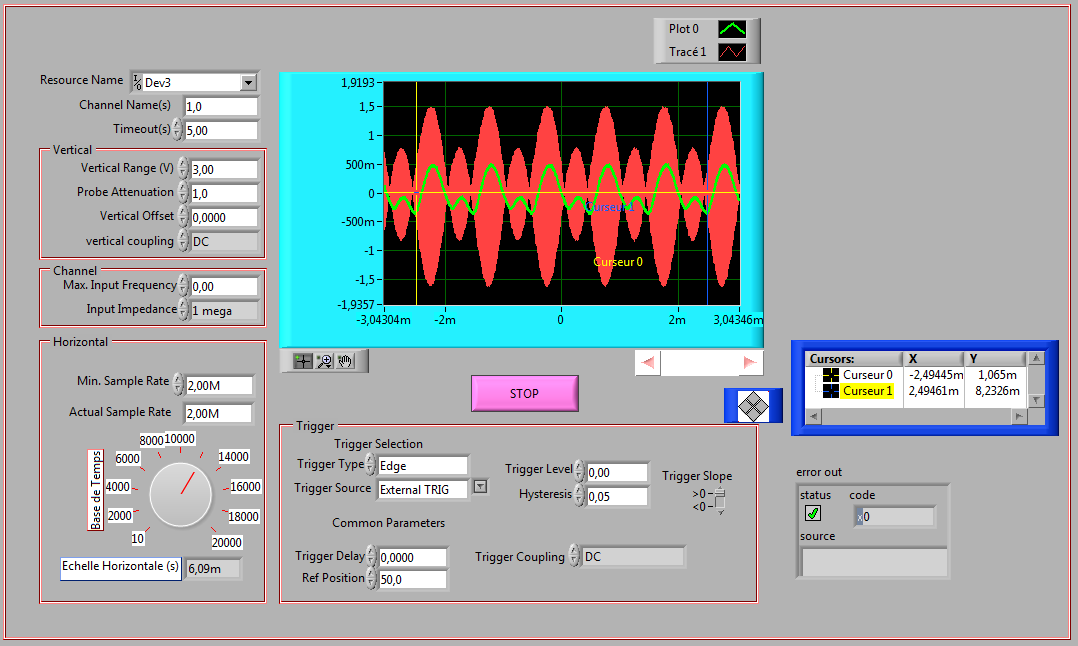
\includegraphics[width=\textwidth]{enveloppe.png}
\item démodulation synchrone : \\
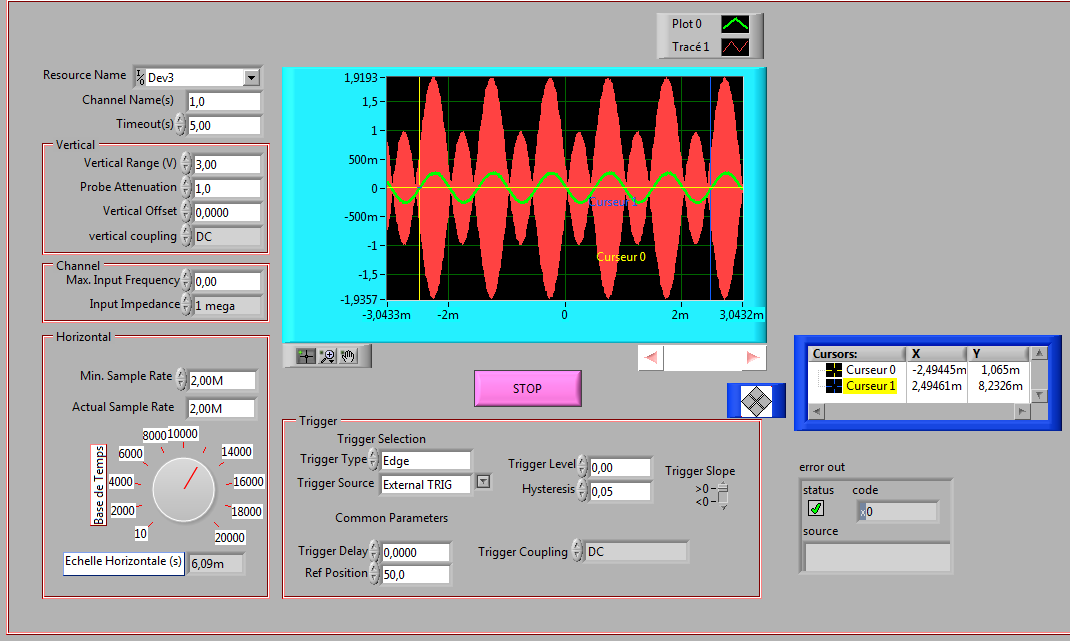
\includegraphics[width=\textwidth]{synchrone.png}
\end{itemize}

\paragraph{Question 7} : \\
Considérons tout d'abord le cas d'un
\subparagraph{Pour un message carré} : \\

\subparagraph{Pour un message triangulaire} : \\

\paragraph{Question 8} : \\

\paragraph{Question 9} : \\



\end{document}